% Created 2013-03-04 lun 22:54
\documentclass[xcolor={usenames,svgnames,dvipsnames}]{beamer}
\usepackage[utf8]{inputenc}
\usepackage[T1]{fontenc}
\usepackage{fixltx2e}
\usepackage{graphicx}
\usepackage{longtable}
\usepackage{float}
\usepackage{wrapfig}
\usepackage{soul}
\usepackage{textcomp}
\usepackage{marvosym}
\usepackage{wasysym}
\usepackage{latexsym}
\usepackage{amssymb}
\usepackage{hyperref}
\tolerance=1000
\usepackage{color}
\usepackage{listings}
\AtBeginSection[]{\begin{frame}<beamer>\frametitle{Contenidos}\tableofcontents[currentsection]\end{frame}}
\lstset{keywordstyle=\color{blue}, commentstyle=\color{gray!90}, basicstyle=\ttfamily\small, columns=fullflexible, breaklines=true,linewidth=\textwidth, backgroundcolor=\color{gray!23}, basewidth={0.5em,0.4em}, literate={á}{{\'a}}1 {ñ}{{\~n}}1 {é}{{\'e}}1 {ó}{{\'o}}1 {º}{{\textordmasculine}}1}
\usepackage{mathpazo}
\setbeamercovered{transparent}
\usefonttheme{serif} 
\usetheme{Goettingen}
\hypersetup{colorlinks=true, linkcolor=Blue, urlcolor=Blue}
\usepackage{fancyvrb}
\DefineVerbatimEnvironment{verbatim}{Verbatim}{fontsize=\tiny, formatcom = {\color{black!70}}}
\providecommand{\alert}[1]{\textbf{#1}}

\title{Gráficos con R}
\author{Oscar Perpiñán Lamigueiro}
\date{Febrero de 2013}
\hypersetup{
  pdfkeywords={},
  pdfsubject={},
  pdfcreator={Emacs Org-mode version 7.8.11}}

\begin{document}

\maketitle




\section{Introducción}
\label{sec-1}
\subsection{Base y grid}
\label{sec-1-1}
\begin{frame}
\frametitle{Base y grid}
\label{sec-1-1-1}

 En \texttt{R} existen dos formas de generar gráficos:
\begin{itemize}
\item Base graphics
\item Grid graphics
\end{itemize}

Dentro del conjunto \texttt{grid} existen dos grandes paquetes:
\begin{itemize}
\item \texttt{lattice}
\item \texttt{ggplot2}
\end{itemize}
\end{frame}
\begin{frame}[fragile]
\frametitle{Conjunto de datos de ejemplo}
\label{sec-1-1-2}

\begin{itemize}
\item Leemos desde el archivo local
\end{itemize}

\lstset{language=R}
\begin{lstlisting}
aranjuez <- read.csv('data/aranjuez.csv')

summary(aranjuez)
\end{lstlisting}


\begin{verbatim}
         X           TempAvg          TempMax          TempMin       
2004-01-01:   1   Min.   :-5.309   Min.   :-2.362   Min.   :-12.980  
2004-01-02:   1   1st Qu.: 7.692   1st Qu.:14.530   1st Qu.:  1.515  
2004-01-03:   1   Median :13.810   Median :21.670   Median :  7.170  
2004-01-04:   1   Mean   :14.405   Mean   :22.531   Mean   :  6.888  
2004-01-05:   1   3rd Qu.:21.615   3rd Qu.:30.875   3rd Qu.: 12.590  
2004-01-06:   1   Max.   :30.680   Max.   :41.910   Max.   : 22.710  
(Other)   :2892                                     NA's   :4        
   HumidAvg         HumidMax         WindAvg         WindMax      
Min.   : 19.89   Min.   : 35.88   Min.   :0.251   Min.   : 0.000  
1st Qu.: 47.04   1st Qu.: 81.60   1st Qu.:0.667   1st Qu.: 3.783  
Median : 62.58   Median : 90.90   Median :0.920   Median : 5.027  
Mean   : 62.16   Mean   : 87.22   Mean   :1.174   Mean   : 5.208  
3rd Qu.: 77.38   3rd Qu.: 94.90   3rd Qu.:1.431   3rd Qu.: 6.537  
Max.   :100.00   Max.   :100.00   Max.   :8.260   Max.   :10.000  
                 NA's   :13       NA's   :8       NA's   :128     
     Rain          Radiation            ET       
Min.   : 0.000   Min.   : 0.277   Min.   :0.000  
1st Qu.: 0.000   1st Qu.: 9.370   1st Qu.:1.168  
Median : 0.000   Median :16.660   Median :2.758  
Mean   : 1.094   Mean   :16.742   Mean   :3.091  
3rd Qu.: 0.200   3rd Qu.:24.650   3rd Qu.:4.926  
Max.   :49.730   Max.   :32.740   Max.   :8.564  
NA's   :4        NA's   :13       NA's   :18
\end{verbatim}
\end{frame}
\begin{frame}[fragile]
\frametitle{Conjunto de datos de ejemplo}
\label{sec-1-1-3}

\begin{itemize}
\item Añadimos algunas columnas
\end{itemize}

\lstset{language=R}
\begin{lstlisting}
aranjuez$month <- as.numeric(
                  format(as.Date(aranjuez$X), '%m'))
aranjuez$year <- as.numeric(
                 format(as.Date(aranjuez$X), '%Y'))
aranjuez$day <- as.numeric(
                format(as.Date(aranjuez$X), '%j'))
aranjuez$jday <- julian(as.Date(aranjuez$X))
aranjuez$quarter <- quarters(as.Date(aranjuez$X))
\end{lstlisting}
\end{frame}
\section{Grid}
\label{sec-2}
\subsection{Lattice}
\label{sec-2-1}
\begin{frame}[fragile]
\frametitle{Lattice}
\label{sec-2-1-1}


\begin{itemize}
\item Documentación: \href{http://lmdvr.r-forge.r-project.org/figures/figures.html}{Código y Figuras del libro}
\end{itemize}


\lstset{language=R}
\begin{lstlisting}
library(lattice)
\end{lstlisting}
\end{frame}
\begin{frame}[fragile]
\frametitle{\texttt{xyplot}}
\label{sec-2-1-2}


\lstset{language=R}
\begin{lstlisting}
xyplot(Radiation ~ TempAvg, data=aranjuez)
\end{lstlisting}

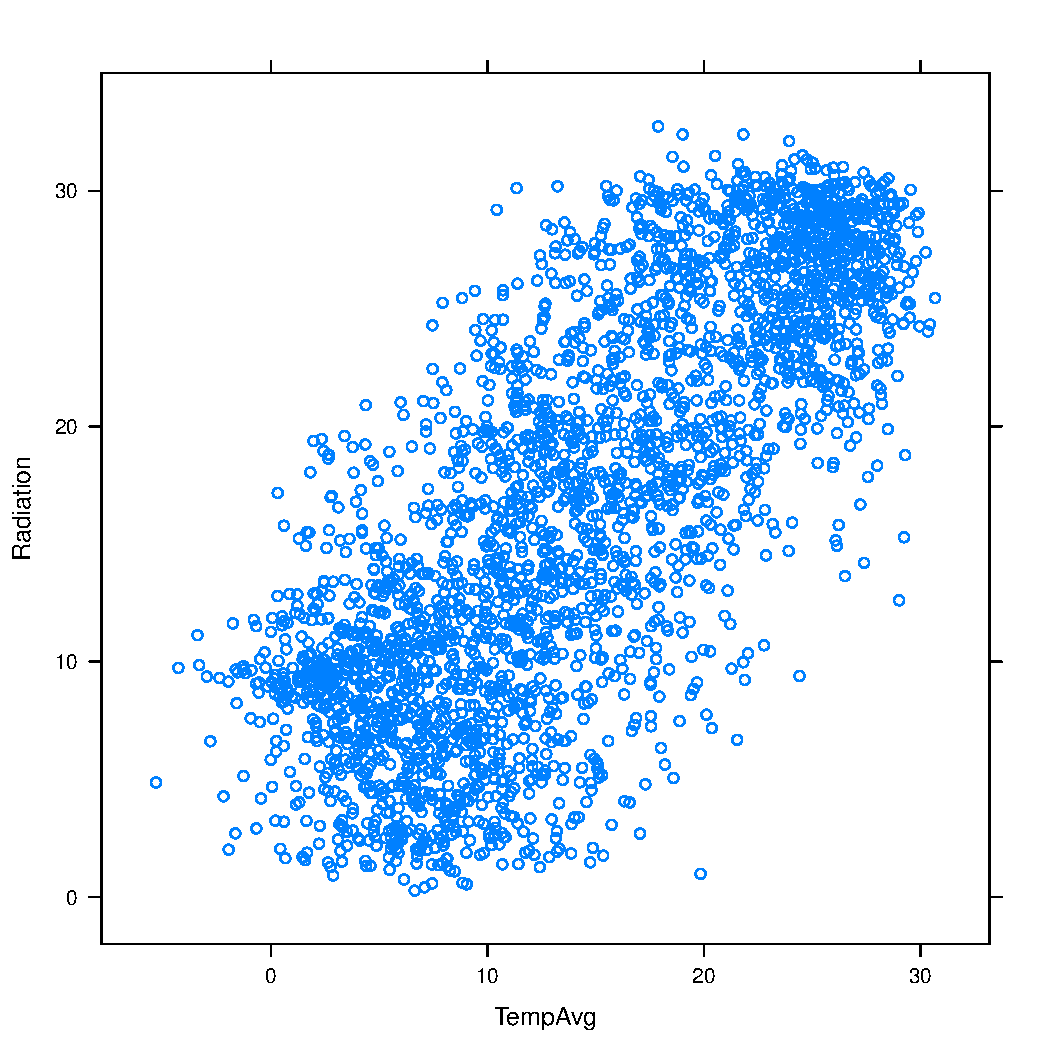
\includegraphics[width=0.7\textwidth]{xyplot.pdf}
\end{frame}
\begin{frame}[fragile]
\frametitle{\texttt{xyplot}}
\label{sec-2-1-3}


\lstset{language=R}
\begin{lstlisting}
xyplot(Radiation ~ TempAvg, data=aranjuez,
       type=c('p', 'g'))
\end{lstlisting}

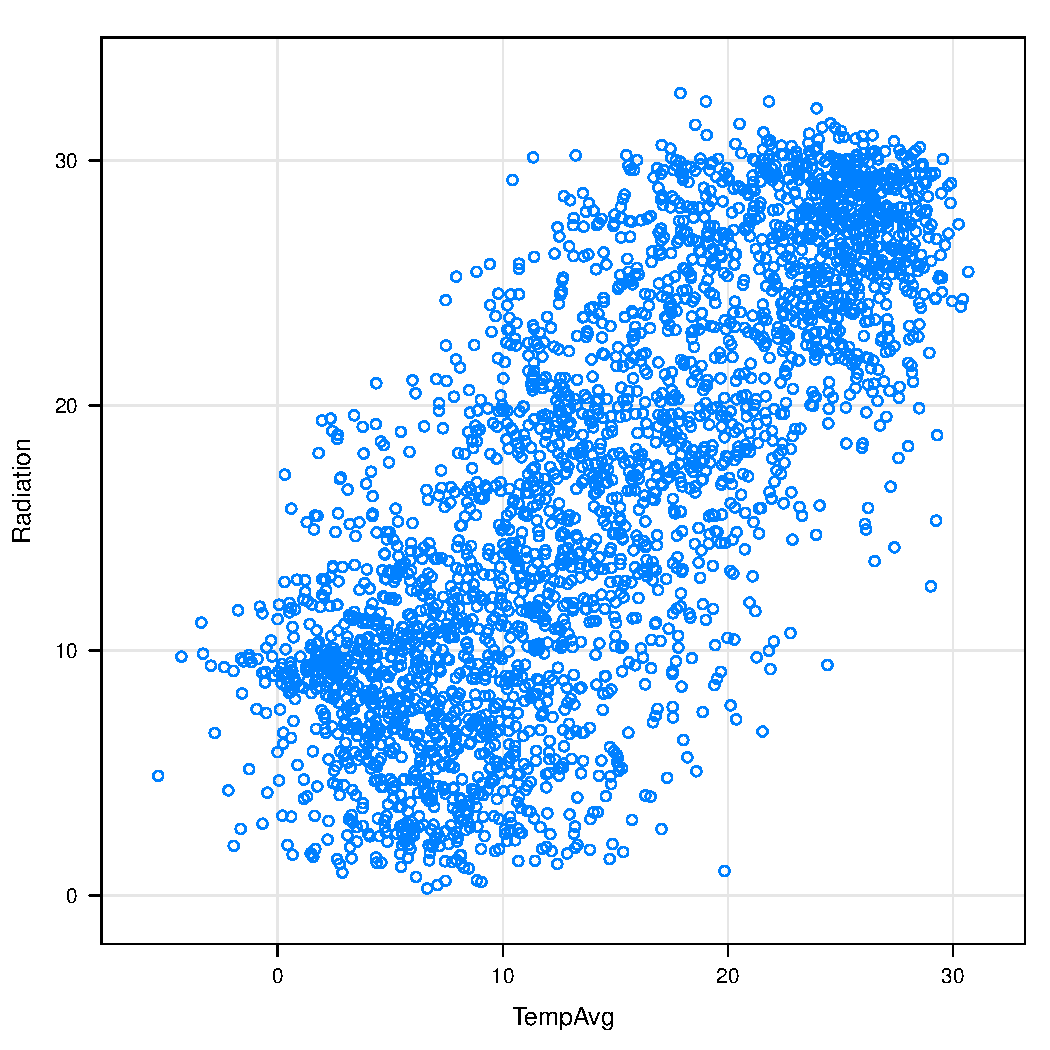
\includegraphics[width=0.7\textwidth]{xyplotPG.pdf}
\end{frame}
\begin{frame}[fragile]
\frametitle{\texttt{xyplot}}
\label{sec-2-1-4}


\lstset{language=R}
\begin{lstlisting}
xyplot(Radiation ~ TempAvg, data=aranjuez,
       type=c('p', 'r', 'g'),
       lwd=2, col.line='black')
\end{lstlisting}

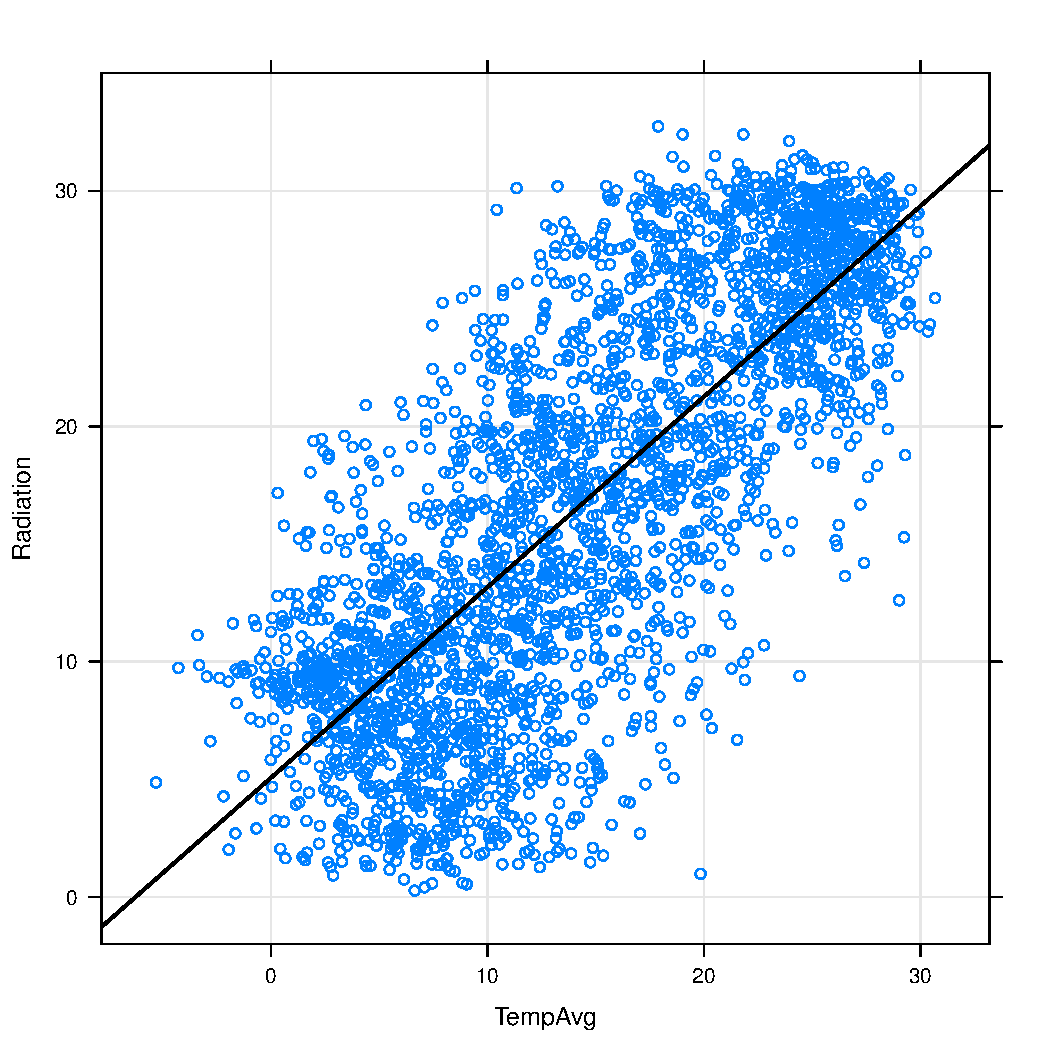
\includegraphics[width=0.7\textwidth]{xyplotPRG.pdf}
\end{frame}
\begin{frame}[fragile]
\frametitle{\texttt{xyplot}}
\label{sec-2-1-5}


\lstset{language=R}
\begin{lstlisting}
xyplot(Radiation ~ TempAvg, data=aranjuez,
       type=c('p', 'smooth', 'g'),
       lwd=2, col.line='black')
\end{lstlisting}

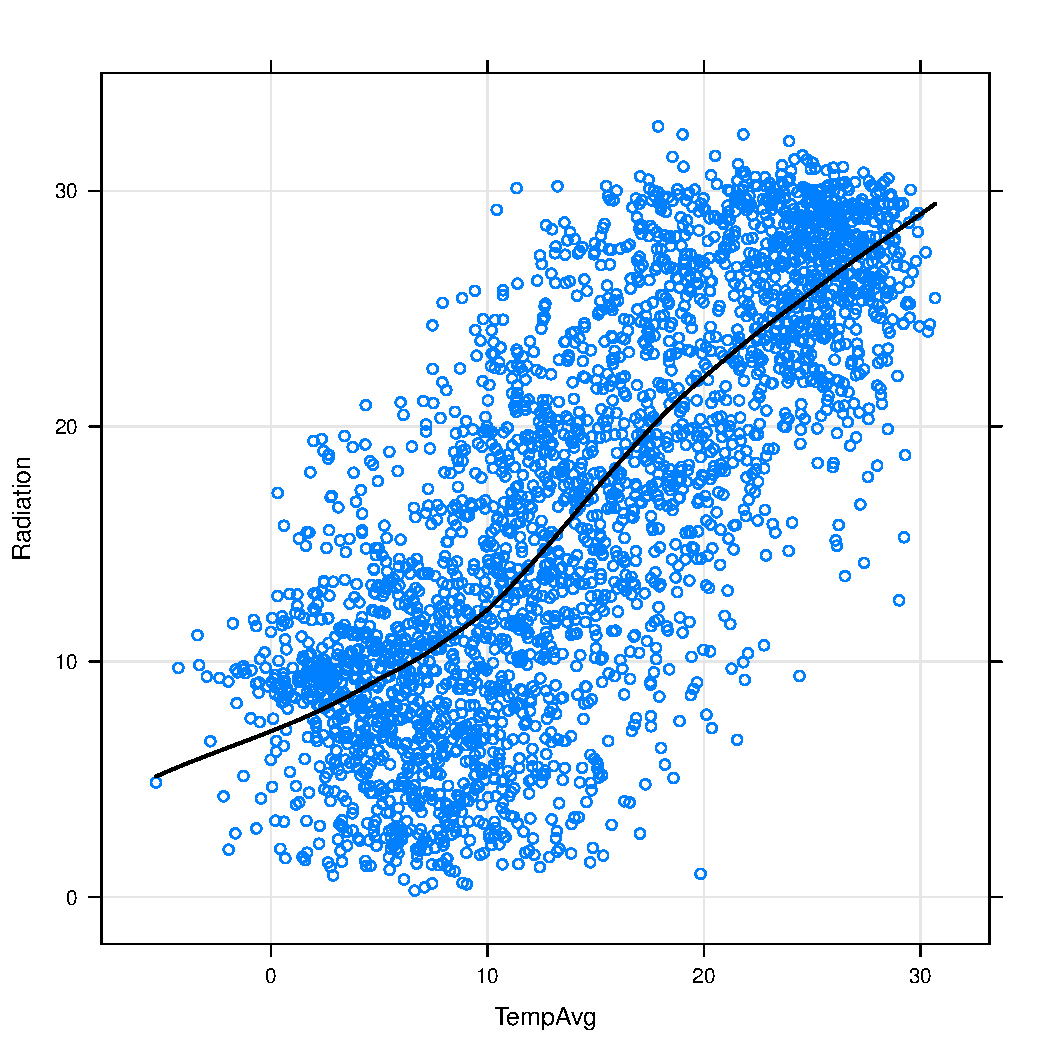
\includegraphics[width=0.7\textwidth]{xyplotSmooth.pdf}
\end{frame}
\begin{frame}[fragile]
\frametitle{Paneles}
\label{sec-2-1-6}


\lstset{language=R}
\begin{lstlisting}
xyplot(Radiation ~ TempAvg|factor(year),
       data=aranjuez)
\end{lstlisting}

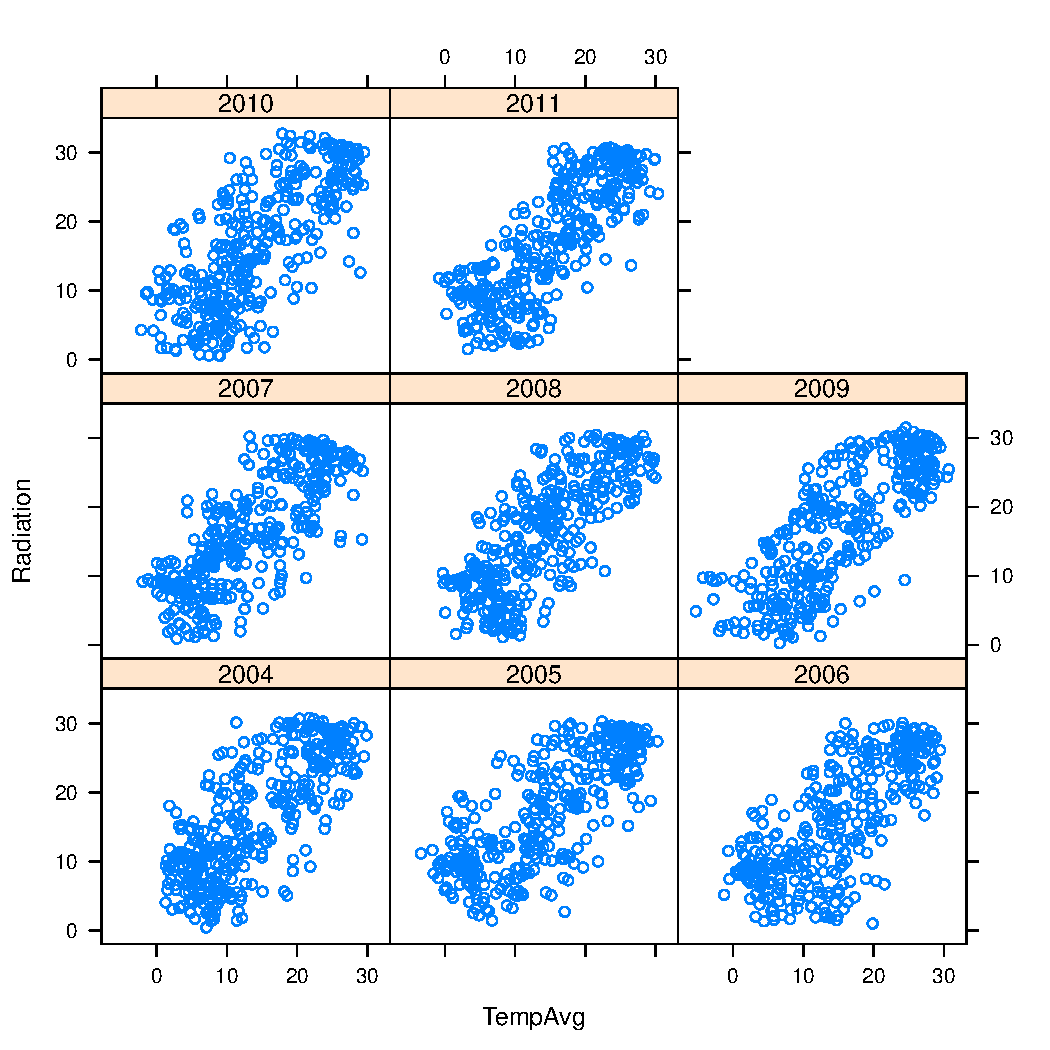
\includegraphics[width=0.7\textwidth]{xyplotYear.pdf}
\end{frame}
\begin{frame}[fragile]
\frametitle{Grupos}
\label{sec-2-1-7}


\lstset{language=R}
\begin{lstlisting}
xyplot(Radiation ~ TempAvg, groups=quarter,
       data=aranjuez, auto.key=list(space='right'))
\end{lstlisting}

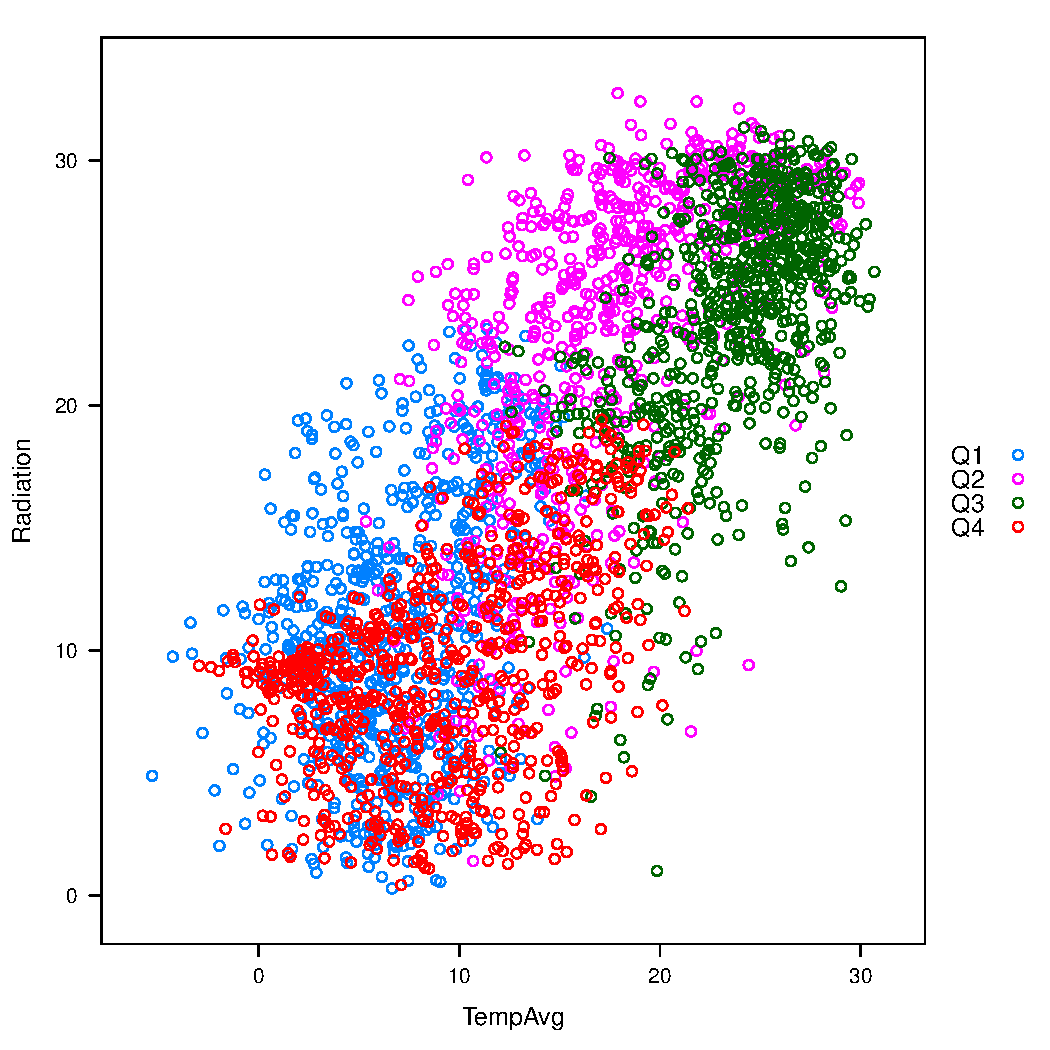
\includegraphics[width=0.7\textwidth]{xyplotQuarter.pdf}
\end{frame}
\begin{frame}[fragile]
\frametitle{Paneles y grupos}
\label{sec-2-1-8}


\lstset{language=R}
\begin{lstlisting}
xyplot(Radiation ~ TempAvg|factor(year),
       groups=quarter,
       data=aranjuez,
       layout=c(4, 2),
       auto.key=list(space='right'))
\end{lstlisting}

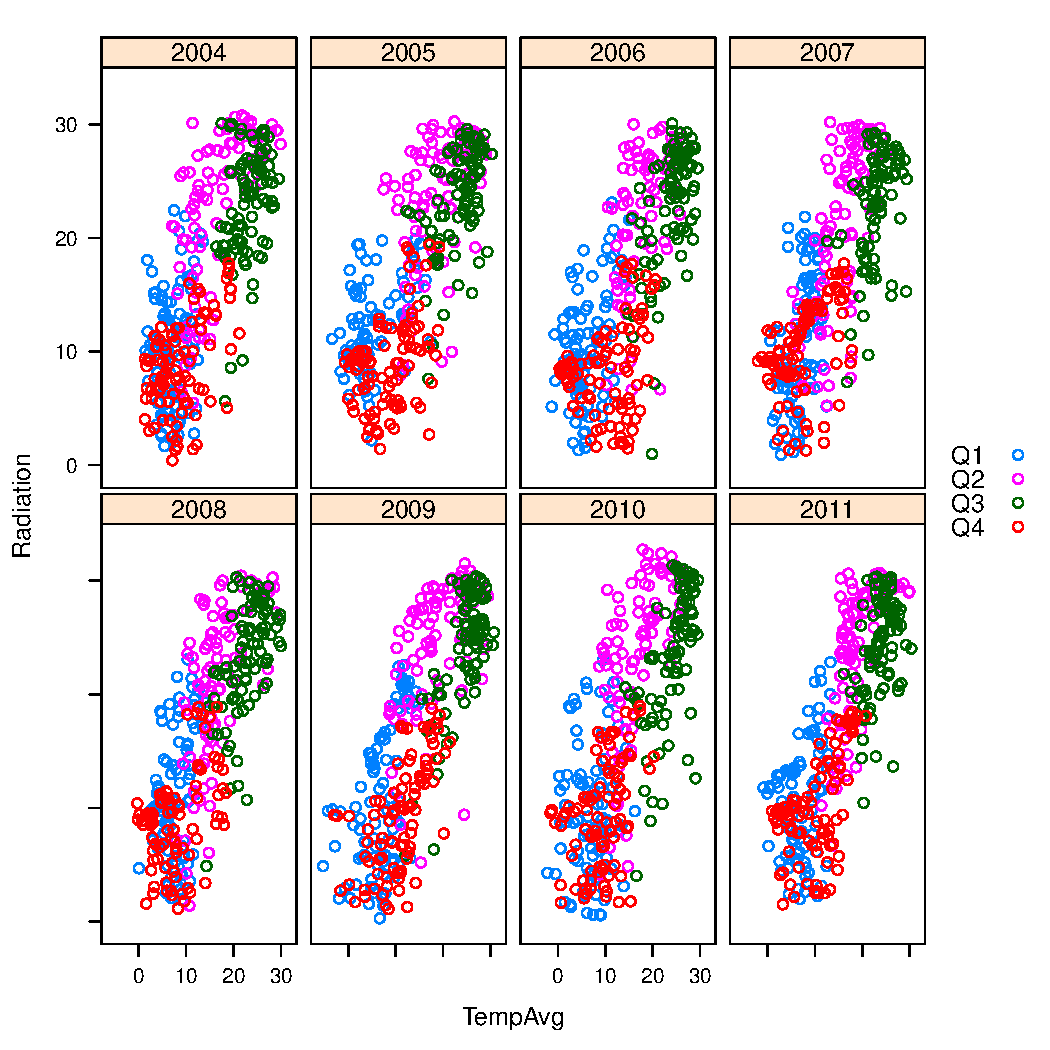
\includegraphics[width=0.6\textwidth]{xyplotQuarterYear.pdf}
\end{frame}
\begin{frame}[fragile]
\frametitle{Paneles y grupos}
\label{sec-2-1-9}


\lstset{language=R}
\begin{lstlisting}
xyplot(Radiation ~ TempAvg|factor(year),
       groups=quarter,
       data=aranjuez,
       layout=c(4, 2),
       type=c('p', 'r'),
       auto.key=list(space='right'))
\end{lstlisting}

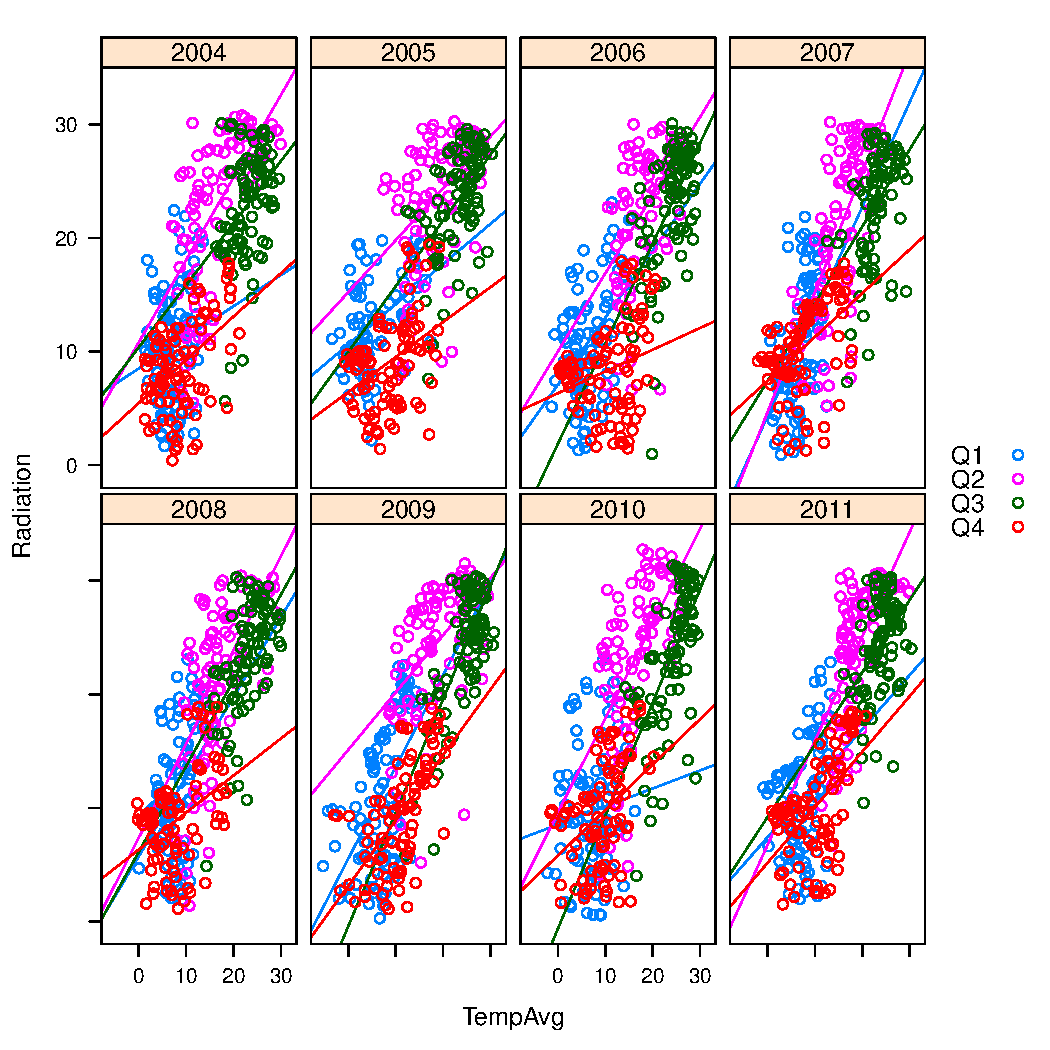
\includegraphics[width=0.6\textwidth]{xyplotQuarterYearSmooth.pdf}
\end{frame}
\begin{frame}[fragile]
\frametitle{Colores y tamaños}
\label{sec-2-1-10}


\lstset{language=R}
\begin{lstlisting}
xyplot(Radiation ~ TempAvg,
       type=c('p', 'r'),
       cex=2, col='blue',
       alpha=.5,
       lwd=3, col.line='black',
       data=aranjuez)
\end{lstlisting}

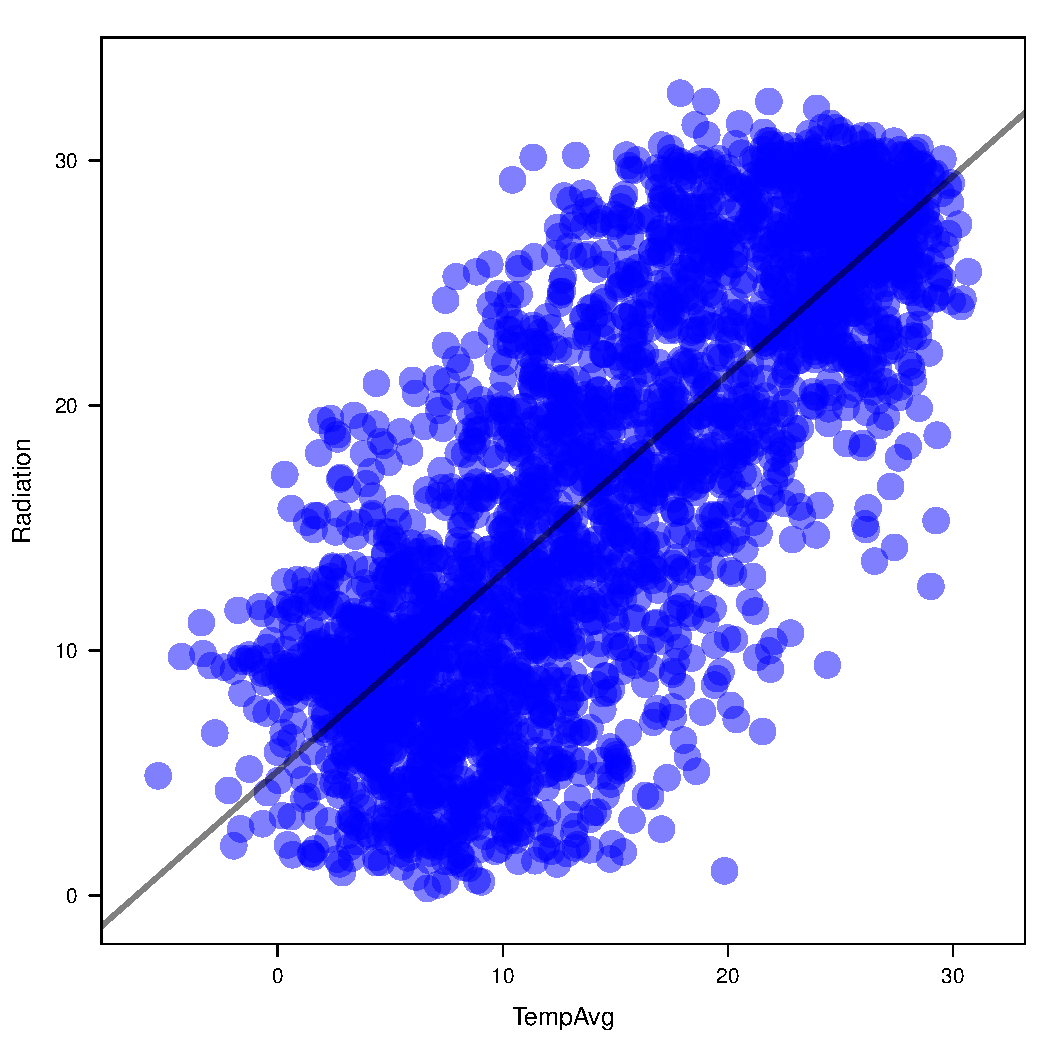
\includegraphics[width=0.6\textwidth]{xyplotColors.pdf}
\end{frame}
\begin{frame}[fragile]
\frametitle{Colores con grupos}
\label{sec-2-1-11}


\lstset{language=R}
\begin{lstlisting}
xyplot(Radiation ~ TempAvg,
       group=quarter,
       col=c('red', 'blue', 'green', 'yellow'),
       auto.key=list(space='right'),
       data=aranjuez)
\end{lstlisting}

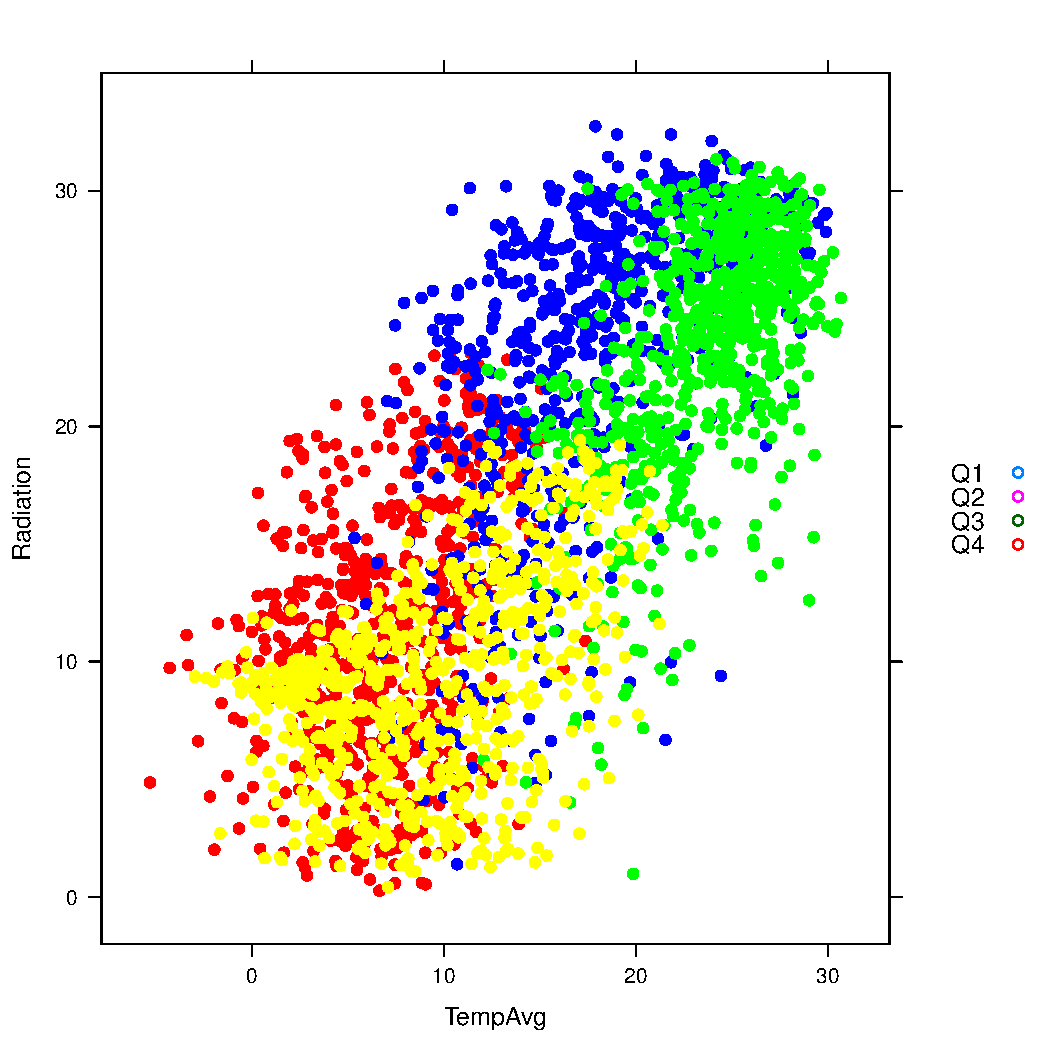
\includegraphics[width=0.6\textwidth]{xyplotColorGroups.pdf}
\end{frame}
\begin{frame}[fragile]
\frametitle{Colores con grupos: par.settings}
\label{sec-2-1-12}


\lstset{language=R}
\begin{lstlisting}
myTheme <- custom.theme(symbol=c('red', 'blue',
                        'green', 'yellow'),
                        pch=19, alpha=.6)
xyplot(Radiation ~ TempAvg,
       groups=quarter,
       par.settings=myTheme,
       auto.key=list(space='right'),
       data=aranjuez)
\end{lstlisting}

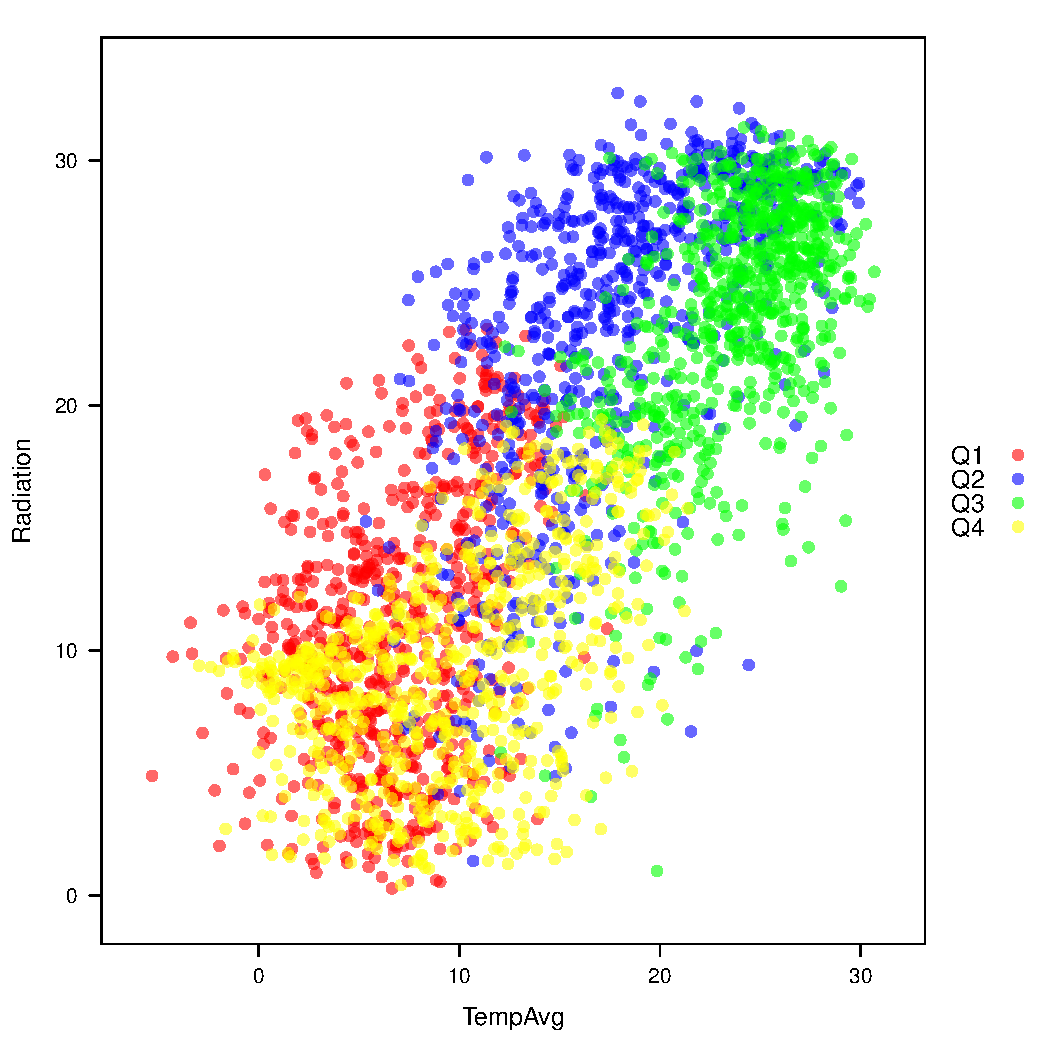
\includegraphics[width=0.45\textwidth]{myTheme.pdf}
\end{frame}
\begin{frame}[fragile]
\frametitle{Colores: brewer.pal}
\label{sec-2-1-13}


\lstset{language=R}
\begin{lstlisting}
library(RColorBrewer)
myTheme <- custom.theme(symbol=brewer.pal(n=4,
                        'Dark2'),
                        pch=19, alpha=.6)
xyplot(Radiation ~ TempAvg,
       groups=quarter,
       par.settings=myTheme,
       auto.key=list(space='right'),
       data=aranjuez)
\end{lstlisting}

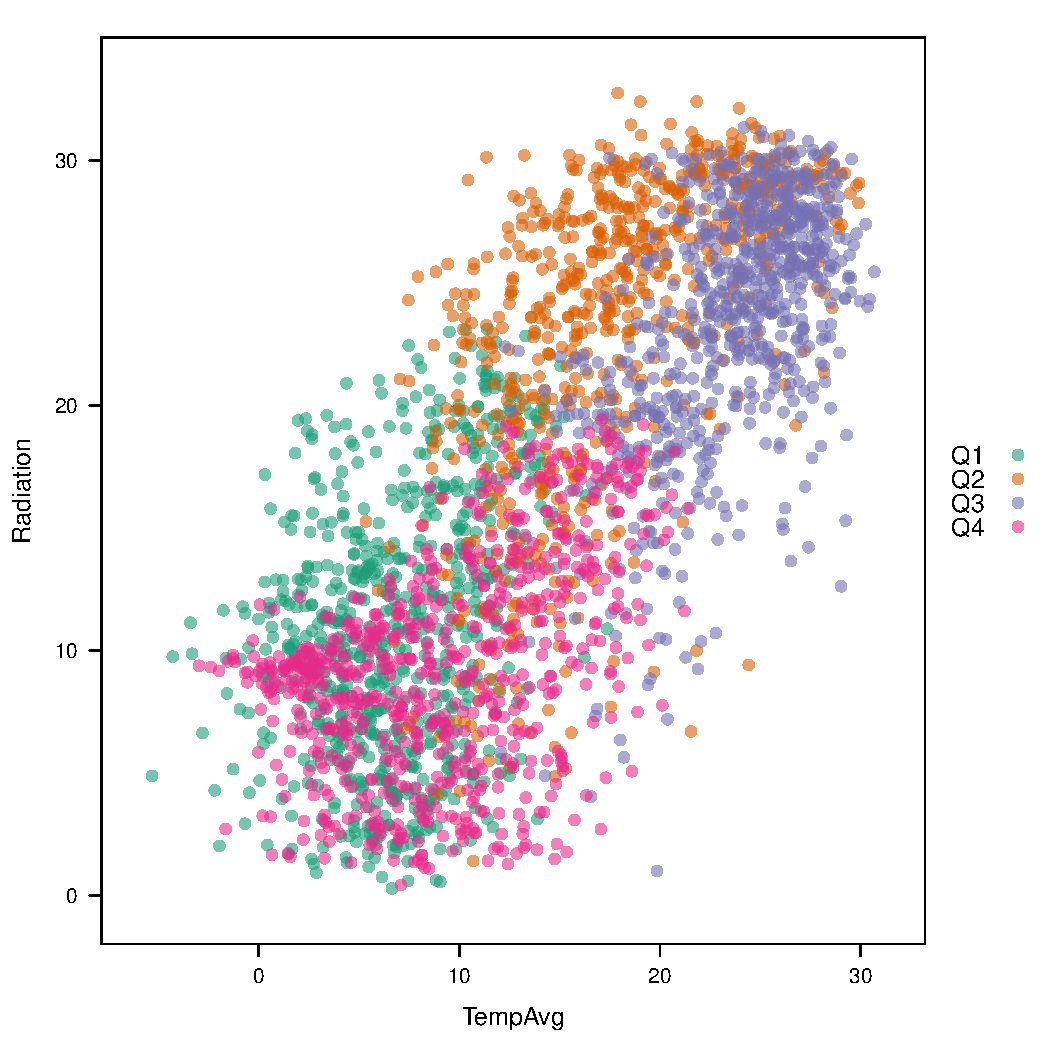
\includegraphics[width=0.45\textwidth]{brewer.pdf}
\end{frame}
\begin{frame}[fragile]
\frametitle{Paneles a medida}
\label{sec-2-1-14}


\lstset{language=R}
\begin{lstlisting}
xyplot(Radiation ~ TempAvg, data=aranjuez,
       panel=function(x, y, ...){
           panel.xyplot(x, y, ...)
           minIdx <- which.min(x)
           maxIdx <- which.max(x)
           panel.points(x[c(minIdx, maxIdx)],
                        y[c(minIdx, maxIdx)],
                        cex=2, col='red')
           panel.text(x[minIdx], y[minIdx],
                      'MIN', pos=1)
           })
\end{lstlisting}

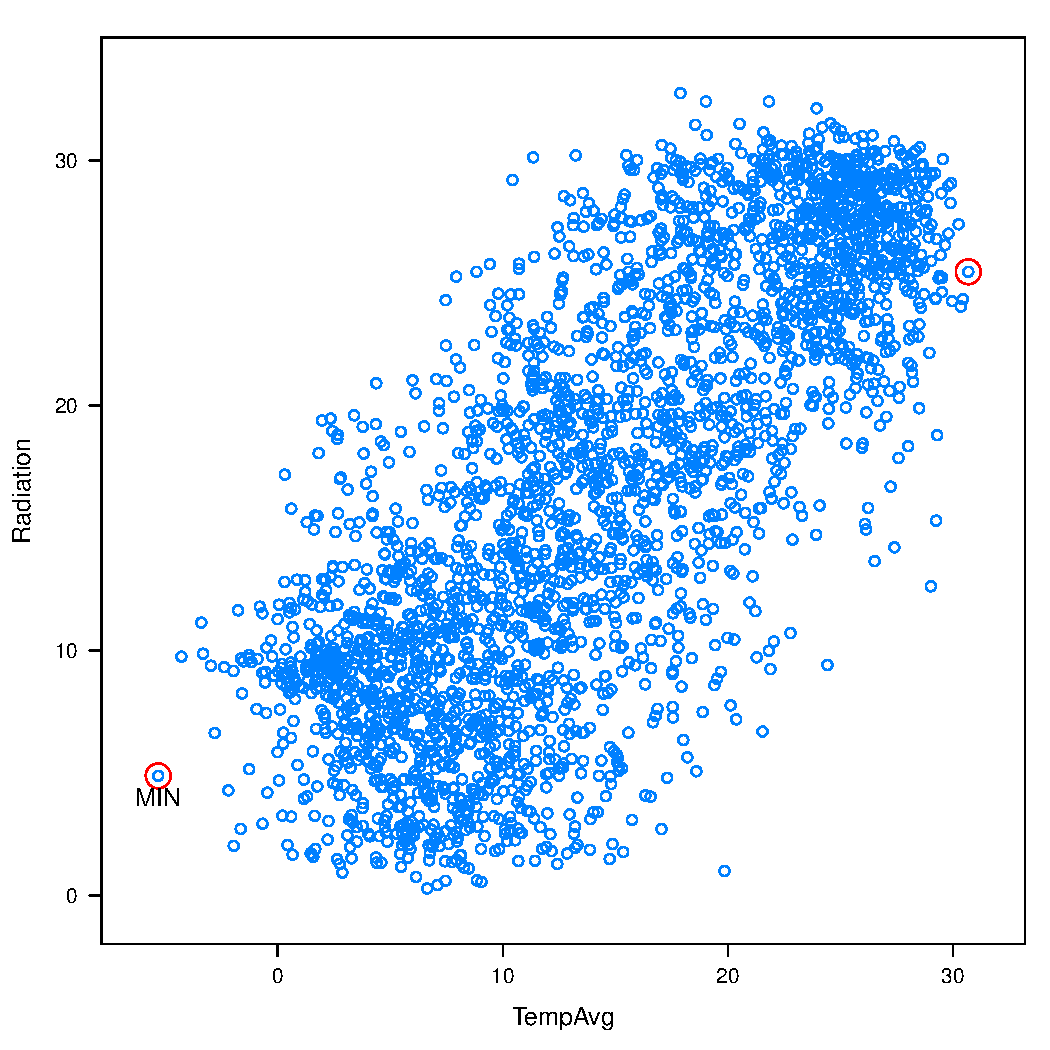
\includegraphics[width=0.3\textwidth]{panel.pdf}
\end{frame}
\begin{frame}[fragile]
\frametitle{Matriz de gráficos de dispersión}
\label{sec-2-1-15}


\lstset{language=R}
\begin{lstlisting}
splom(aranjuez[,c("TempAvg", "HumidAvg", "WindAvg",
                  "Rain", "Radiation", "ET")],
      pscale=0, alpha=0.6, cex=0.3, pch=19)
\end{lstlisting}

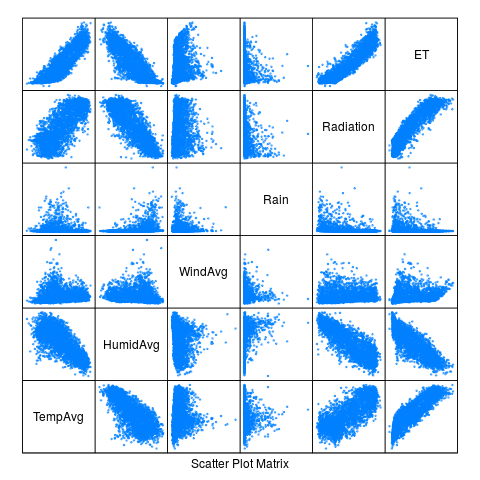
\includegraphics[width=0.45\textwidth]{splom.png}
\end{frame}
\begin{frame}[fragile]
\frametitle{Matriz de gráficos de dispersión}
\label{sec-2-1-16}


\lstset{language=R}
\begin{lstlisting}
splom(aranjuez[,c("TempAvg", "HumidAvg", "WindAvg",
                  "Rain", "Radiation", "ET")],
      groups=aranjuez$quarter,
      auto.key=list(space='right'),
      pscale=0, alpha=0.6, cex=0.3, pch=19)
\end{lstlisting}

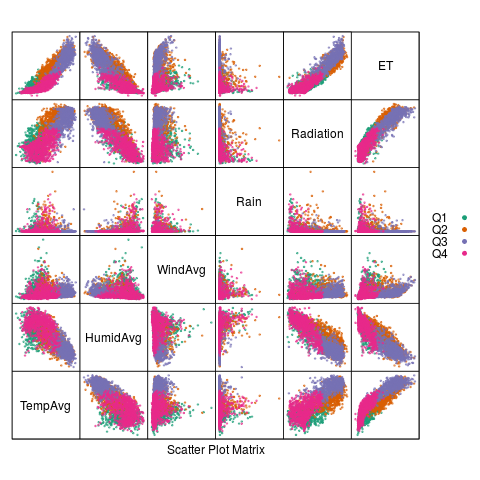
\includegraphics[width=0.45\textwidth]{splomGroup.png}
\end{frame}
\begin{frame}[fragile]
\frametitle{\texttt{levelplot}}
\label{sec-2-1-17}


\lstset{language=R}
\begin{lstlisting}
levelplot(TempAvg ~ year * day,
          data=aranjuez)
\end{lstlisting}

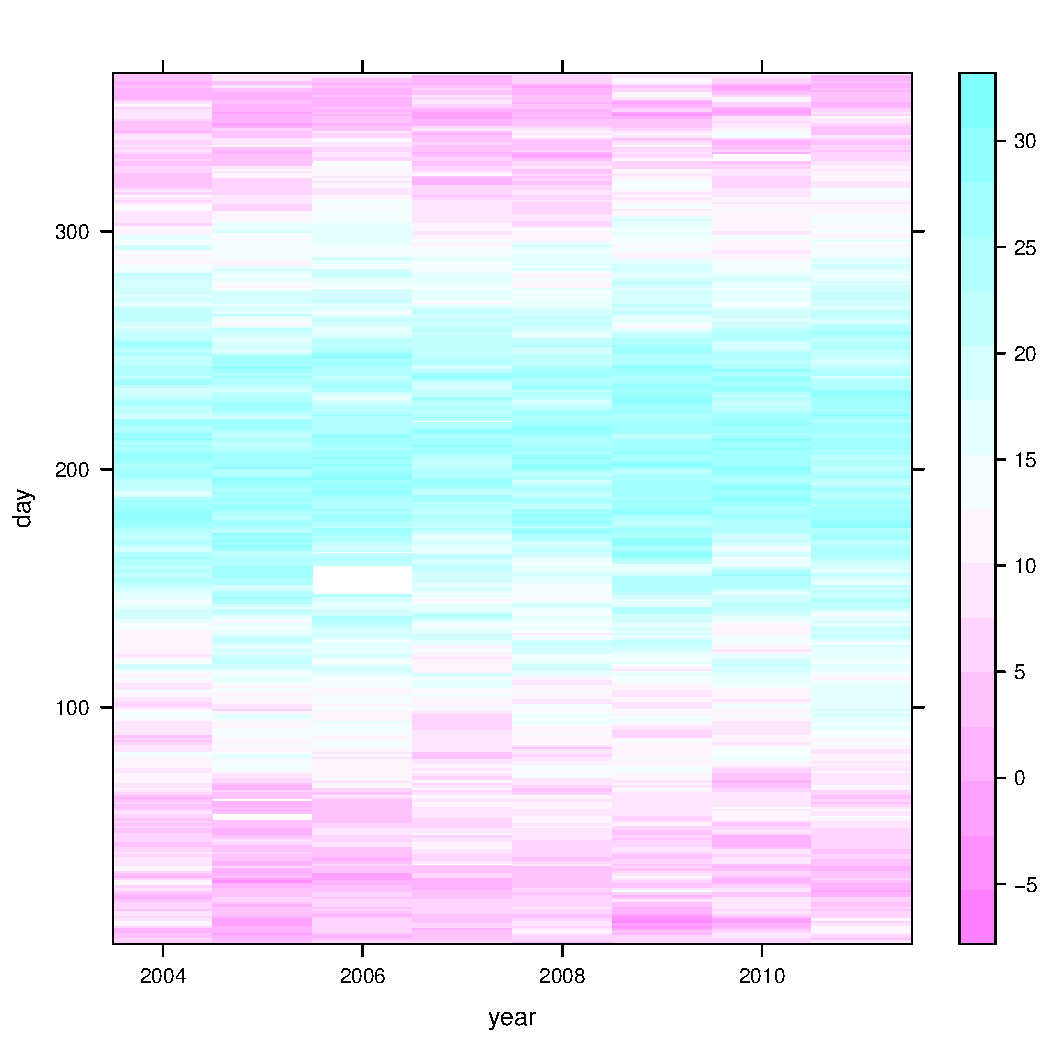
\includegraphics[width=0.6\textwidth]{levelplot.pdf}
\end{frame}
\begin{frame}[fragile]
\frametitle{\texttt{contourplot}}
\label{sec-2-1-18}


\lstset{language=R}
\begin{lstlisting}
contourplot(Radiation ~ year * day,
            lwd=.5, labels=FALSE,
            region=TRUE, 
            data=aranjuez)
\end{lstlisting}

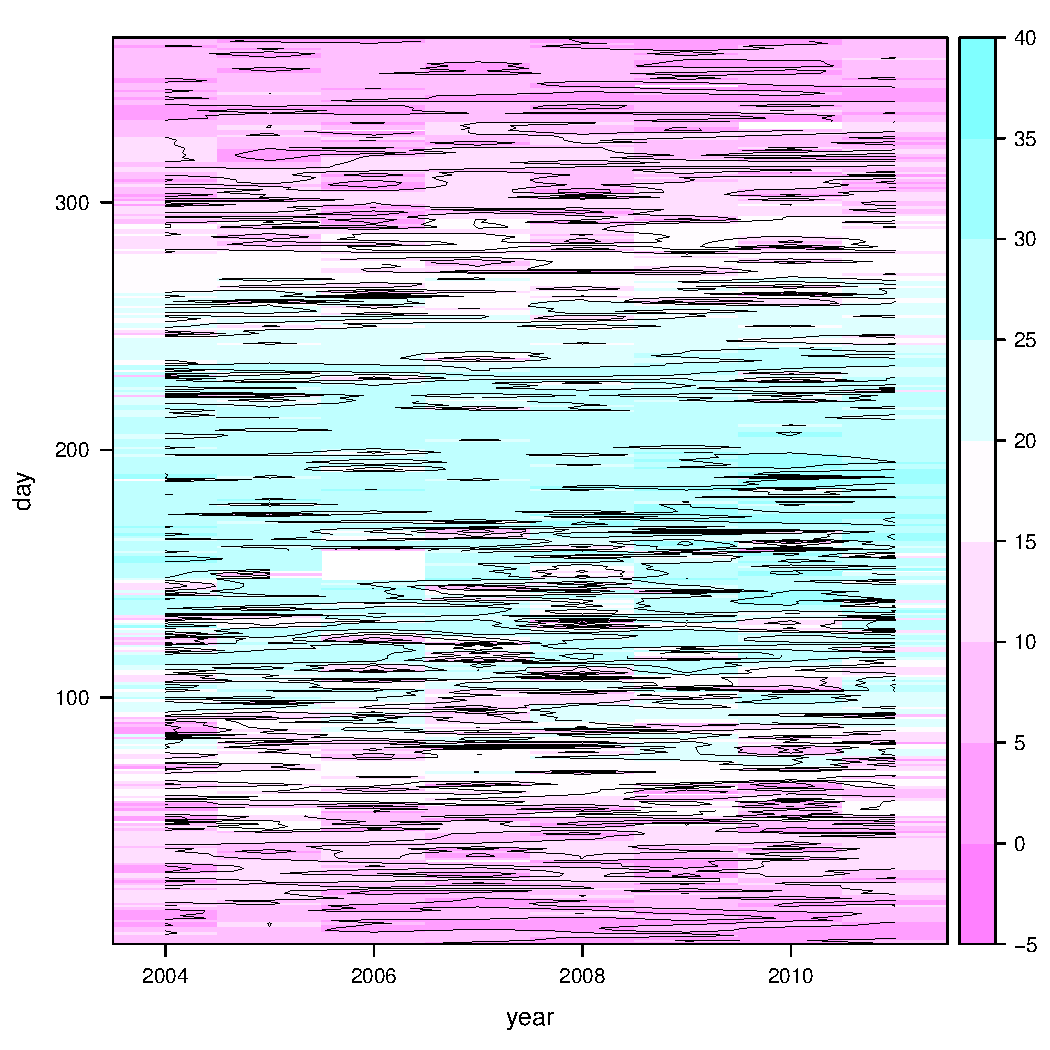
\includegraphics[width=0.7\textwidth]{contourplot.pdf}
\end{frame}
\begin{frame}[fragile]
\frametitle{Box-and-Whiskers}
\label{sec-2-1-19}


\lstset{language=R}
\begin{lstlisting}
bwplot(Radiation ~ month, data=aranjuez,
       horizontal=FALSE, pch='|')
\end{lstlisting}

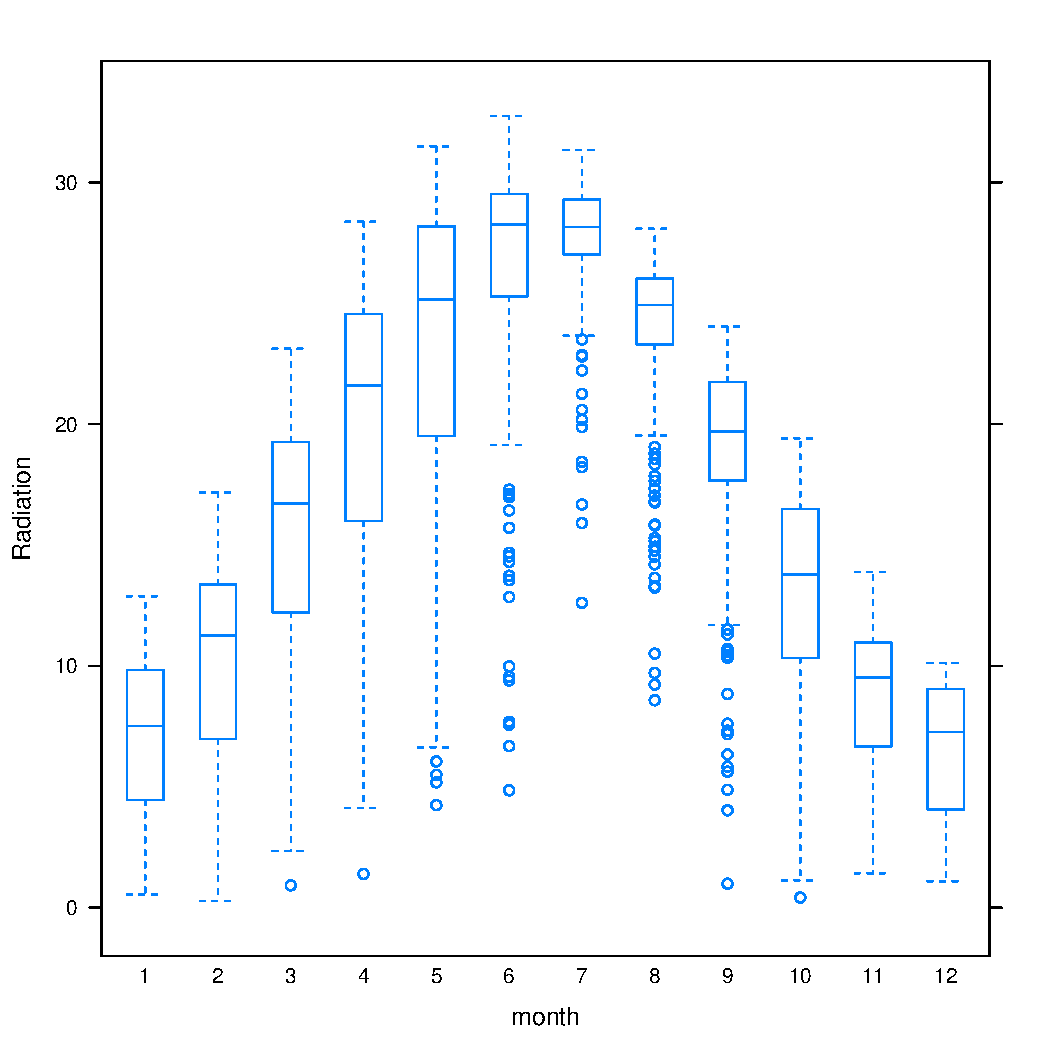
\includegraphics[width=0.7\textwidth]{bwplot.pdf}
\end{frame}
\begin{frame}[fragile]
\frametitle{Box-and-Whiskers}
\label{sec-2-1-20}


\lstset{language=R}
\begin{lstlisting}
bwplot(Radiation ~ month, data=aranjuez,
       horizontal=FALSE,
       panel=panel.violin)
\end{lstlisting}

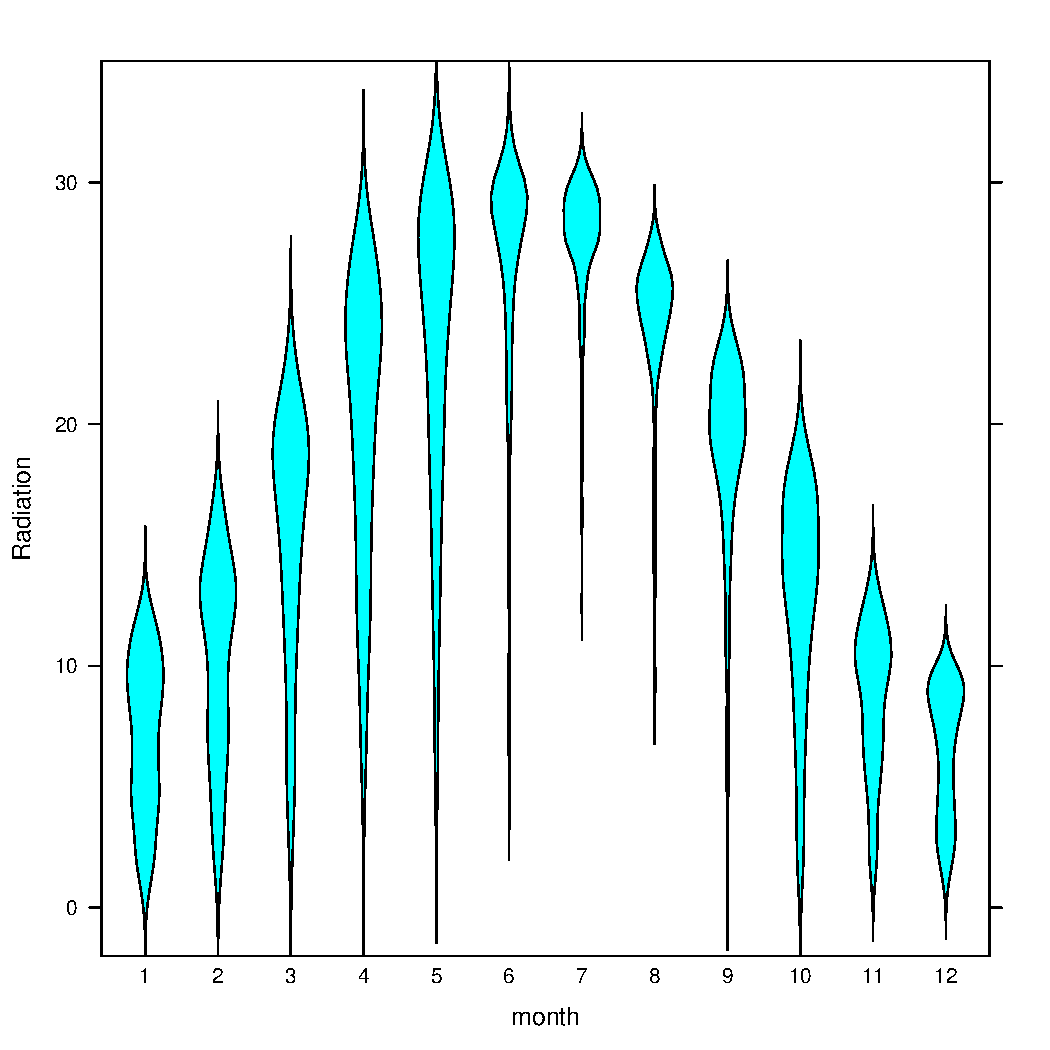
\includegraphics[width=0.7\textwidth]{violin.pdf}

    
\end{frame}
\begin{frame}[fragile]
\frametitle{Histogramas}
\label{sec-2-1-21}


\lstset{language=R}
\begin{lstlisting}
histogram(~Radiation|factor(year), data=aranjuez)
\end{lstlisting}

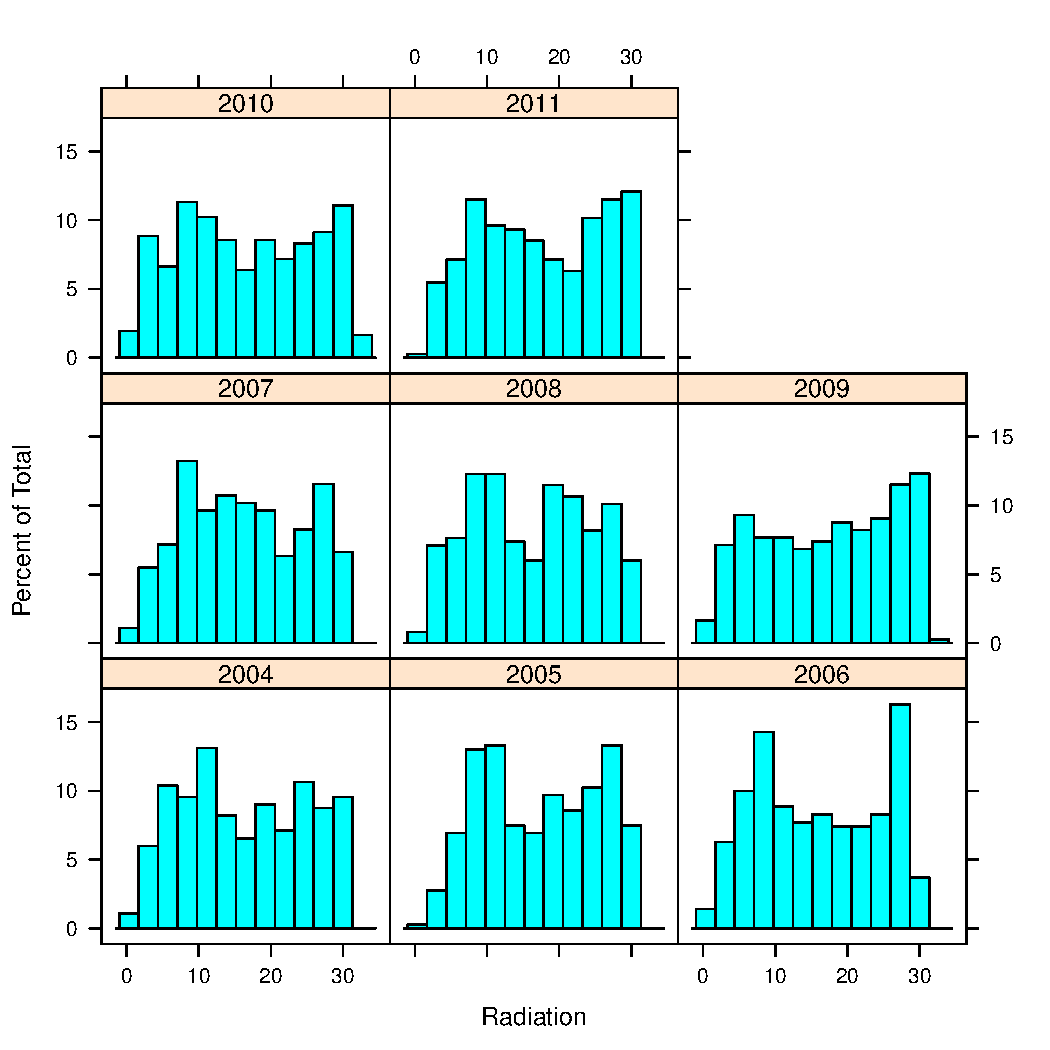
\includegraphics[width=0.7\textwidth]{histogram.pdf}
\end{frame}
\begin{frame}[fragile]
\frametitle{Gráficos de densidad}
\label{sec-2-1-22}


\lstset{language=R}
\begin{lstlisting}
densityplot(~Radiation, groups=quarter,
            data=aranjuez,
            auto.key=list(space='right'))
\end{lstlisting}

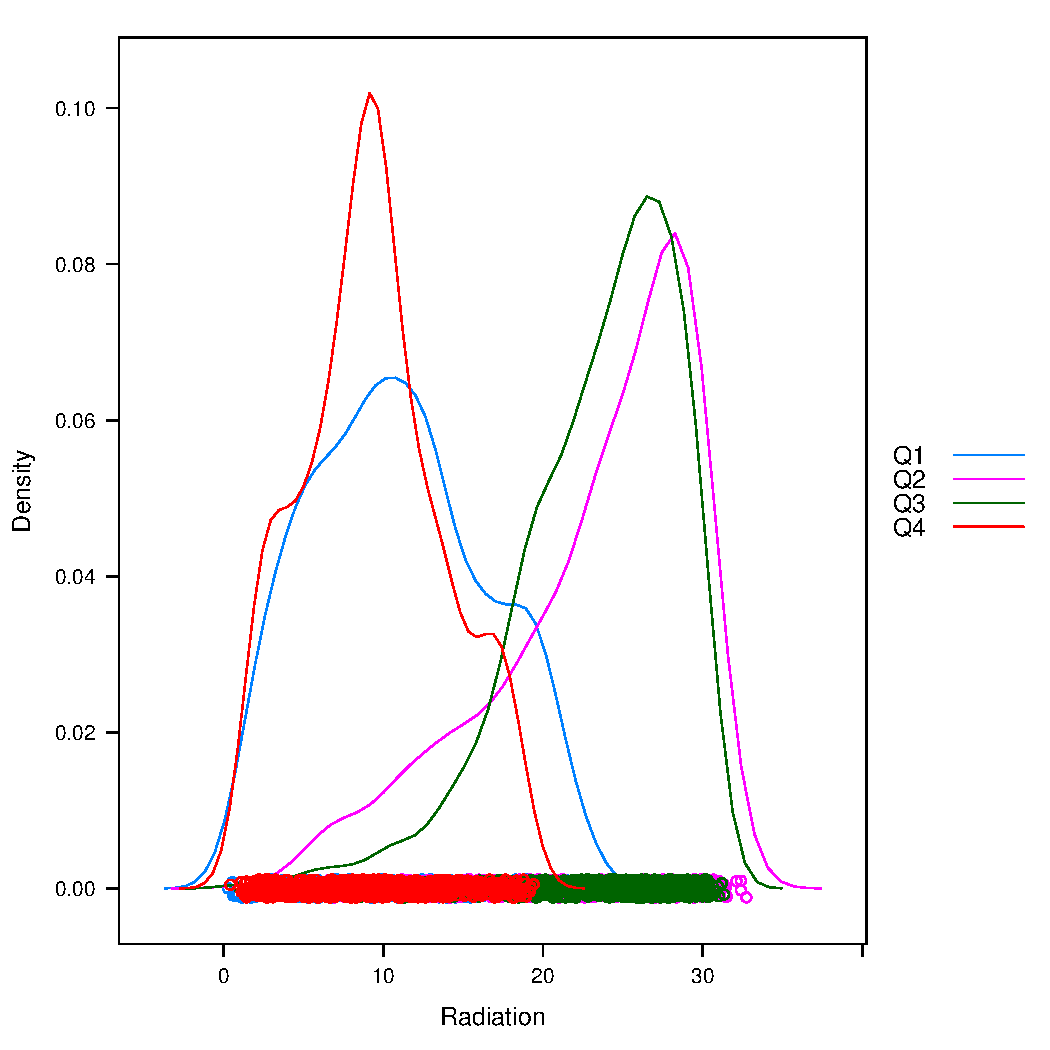
\includegraphics[width=0.7\textwidth]{density.pdf}
\end{frame}
\begin{frame}[fragile]
\frametitle{\texttt{dotplot}}
\label{sec-2-1-23}


\lstset{language=R}
\begin{lstlisting}
avRad <- aggregate(Radiation ~ month * year,
                   data=aranjuez, FUN=mean)
\end{lstlisting}



\lstset{language=R}
\begin{lstlisting}
dotplot(month ~ Radiation|factor(year), data=avRad)
\end{lstlisting}

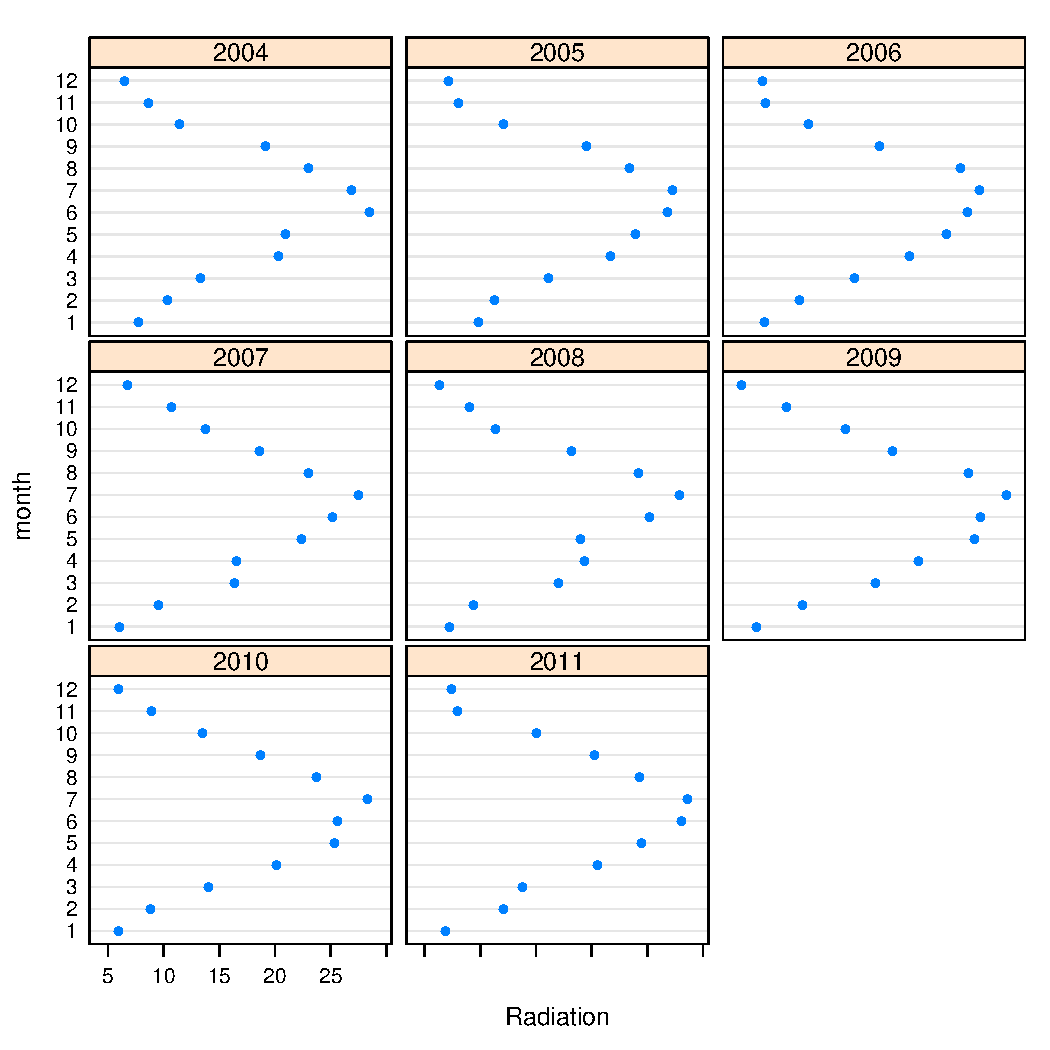
\includegraphics[width=0.7\textwidth]{dotplot.pdf}
\end{frame}
\begin{frame}[fragile]
\frametitle{Quantile-Quantile}
\label{sec-2-1-24}


\lstset{language=R}
\begin{lstlisting}
firstHalf <- aranjuez$quarter %in% c('Q1', 'Q2')

qq(firstHalf ~ Radiation, data=aranjuez)
\end{lstlisting}

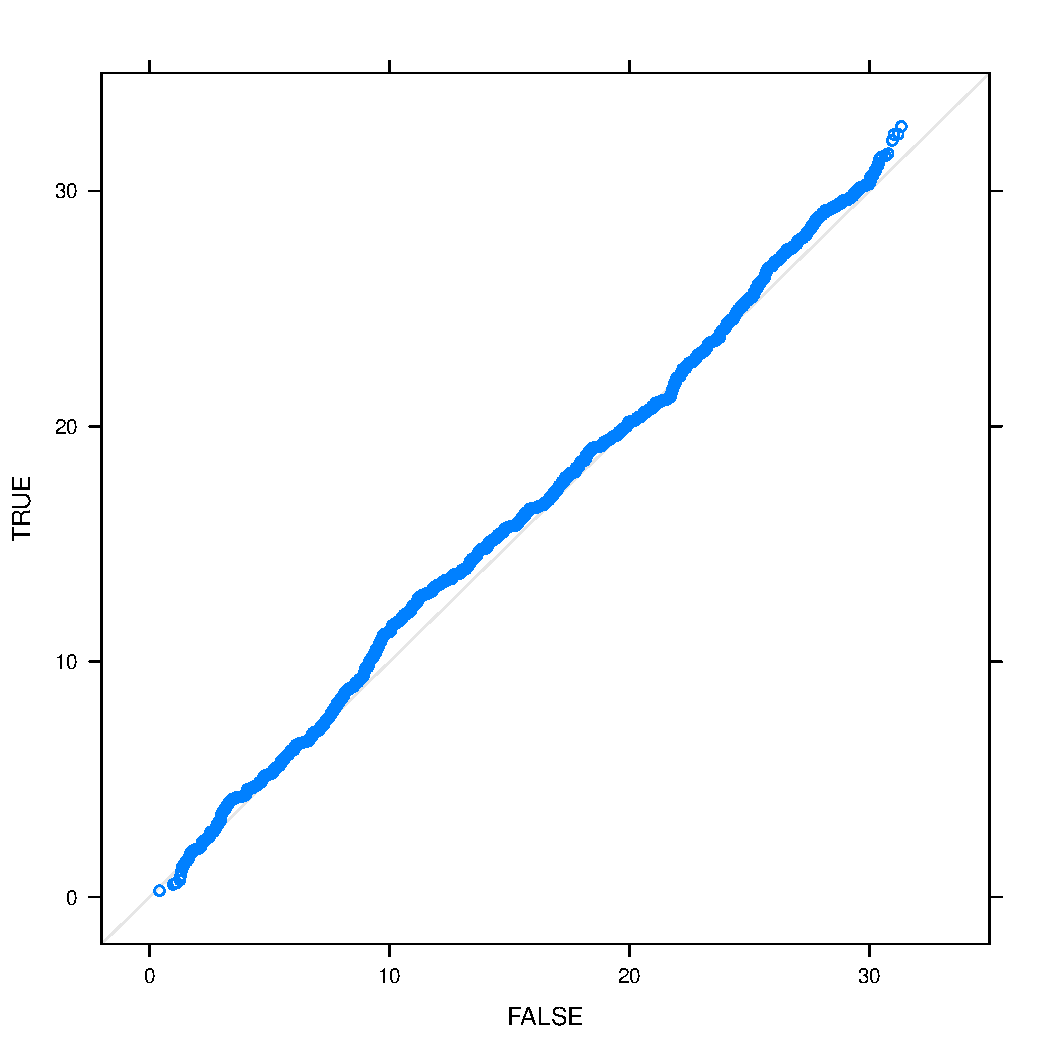
\includegraphics[width=0.7\textwidth]{qqHalf.pdf}
\end{frame}
\begin{frame}[fragile]
\frametitle{Quantile-quantile}
\label{sec-2-1-25}


\lstset{language=R}
\begin{lstlisting}
winter <- aranjuez$quarter %in% c('Q1', 'Q4')

qq(winter ~ Radiation, data=aranjuez)
\end{lstlisting}

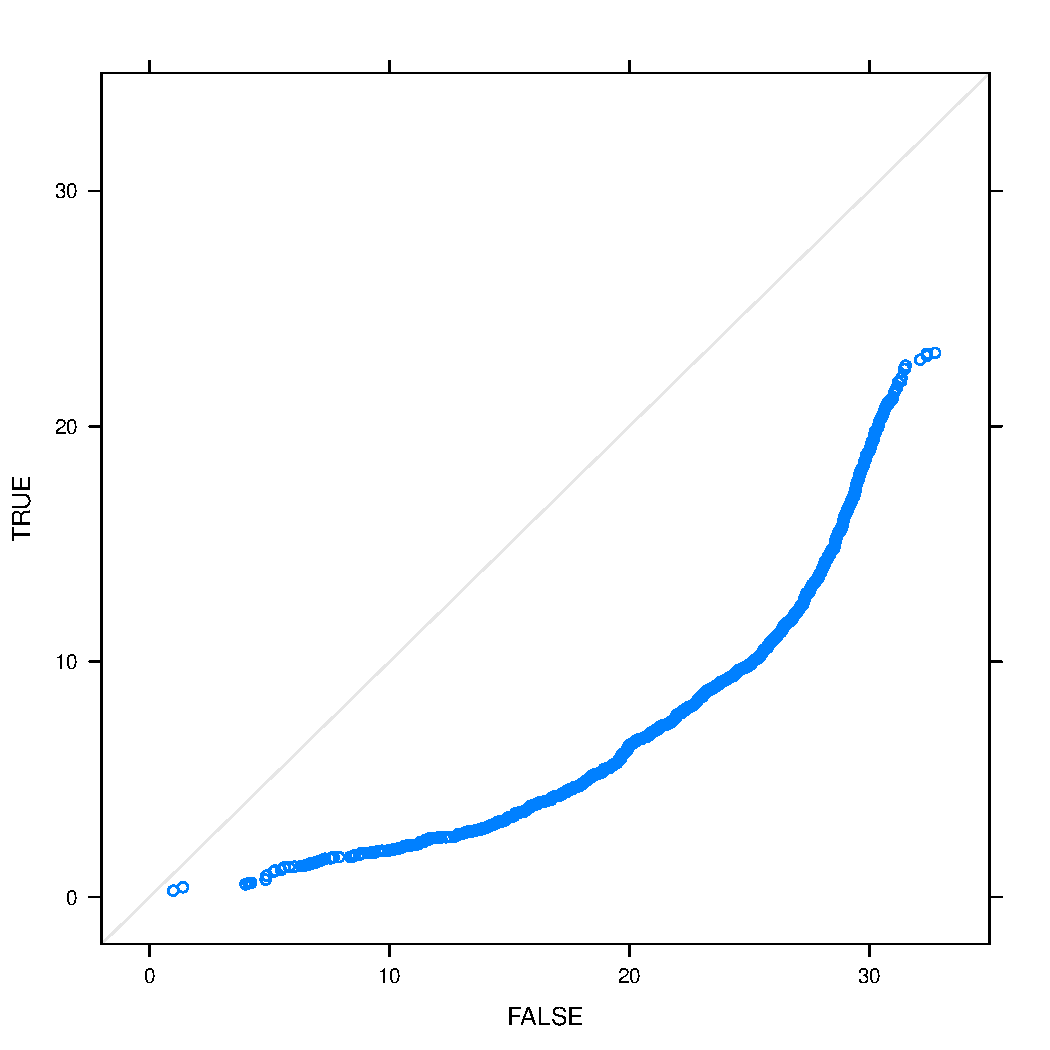
\includegraphics[width=0.7\textwidth]{qqWinter.pdf}
\end{frame}
\begin{frame}[fragile]
\frametitle{Quantile-Quantile}
\label{sec-2-1-26}


\lstset{language=R}
\begin{lstlisting}
qqmath(~TempAvg, data=aranjuez,
       groups=year, distribution=qnorm)
\end{lstlisting}

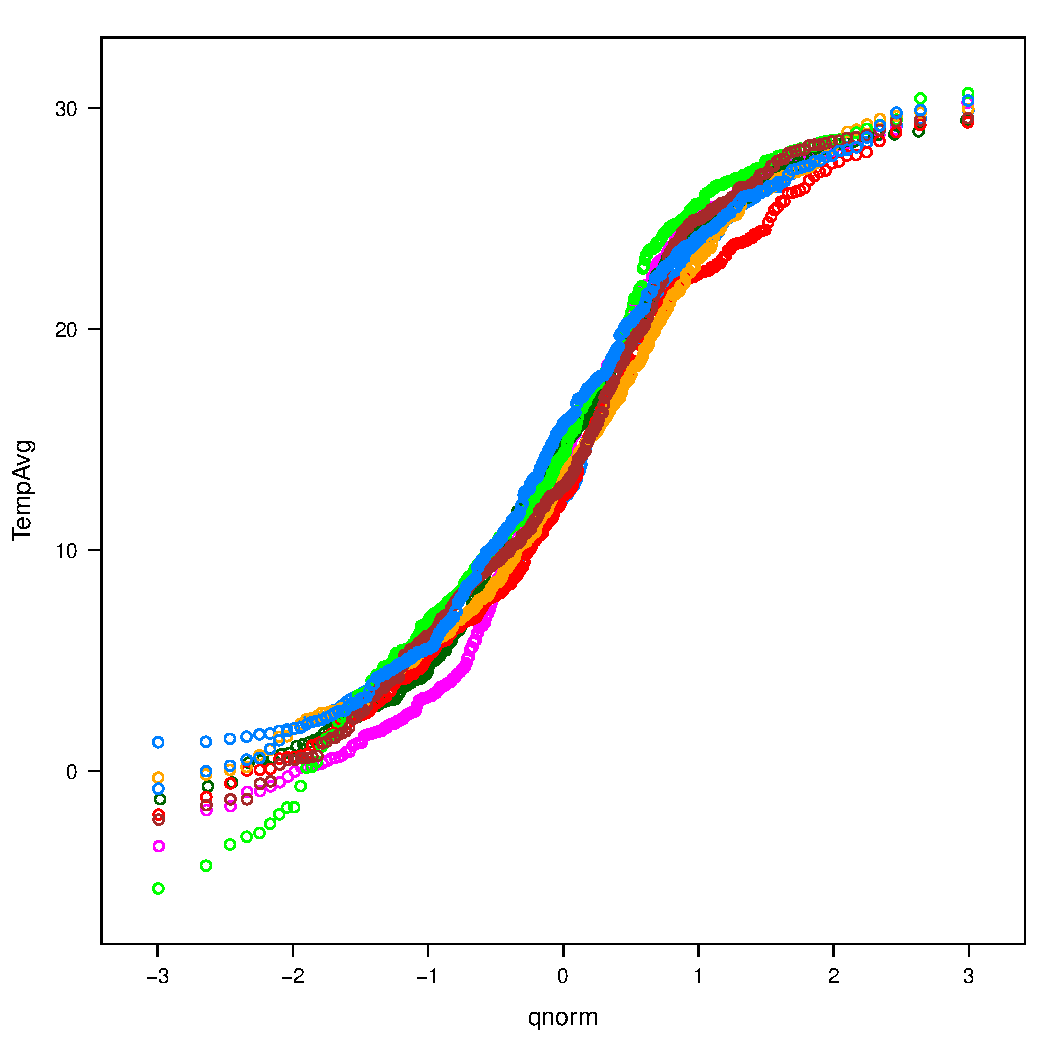
\includegraphics[width=0.7\textwidth]{qqNorm.pdf}
\end{frame}
\subsection{ggplot2}
\label{sec-2-2}
\begin{frame}
\frametitle{ggplot2}
\label{sec-2-2-1}

\begin{itemize}
\item \href{http://docs.ggplot2.org/current/}{Documentación de ggplot2}
\item \href{http://ggplot2.org/book/}{Codigo del libro}
\item \href{http://learnr.wordpress.com/2009/06/28/ggplot2-version-of-figures-in-lattice-multivariate-data-visualization-with-r-part-1/}{ggplot2 desde lattice} (\href{http://learnr.files.wordpress.com/2009/08/latbook.pdf}{PDF})
\end{itemize}
\end{frame}

\end{document}